\documentclass[12pt,a4paper]{article}
\usepackage[utf8]{inputenc}
\usepackage[T1]{fontenc}
\usepackage{times}
\usepackage[margin=1in]{geometry}
\usepackage{graphicx}
\usepackage{xcolor}
\usepackage{hyperref}
\usepackage{listings}
\usepackage{booktabs}
\usepackage{tabularx}
\usepackage{multirow}
\usepackage{amsmath,amssymb}
\usepackage{tikz}
\usetikzlibrary{shapes.geometric, arrows, positioning, shadows}
\usepackage{fancyhdr}
\usepackage{titlesec}
\usepackage{caption}
\usepackage{setspace}
\usepackage{enumitem}

\onehalfspacing

% Hyperref Setup
\hypersetup{
    colorlinks=true,
    linkcolor=black,
    citecolor=black,
    urlcolor=blue,
    pdftitle={DRDO SSPL Internship Report - Trainee & Internship Management Portal},
    pdfauthor={Tarleen Kaur / Trainee},
    pdfsubject={Software Engineering & Web Application Development}
}

% Header & Footer Setup
\pagestyle{fancy}
\fancyhf{}
\fancyhead[L]{\small Solid State Physics Laboratory (SSPL) -- DRDO}
\fancyhead[R]{\small Trainee Management Portal Report}
\fancyfoot[C]{\thepage}
\renewcommand{\headrulewidth}{0.4pt}

% Custom section formatting to match DRDO reference report
\titleformat{\section}[block]{\centering\normalfont\Large\bfseries\uppercase}{}{0pt}{}
\titleformat{\subsection}[block]{\normalfont\large\bfseries}{\thesubsection}{1em}{}
\titleformat{\subsubsection}[block]{\normalfont\bfseries}{\thesubsubsection}{1em}{}

\begin{document}

% ==========================================
% PAGE 1: COVER / TITLE PAGE
% ==========================================
\begin{titlepage}
    \centering
    \vspace*{0.5cm}
    
    {\Large \textbf{INTERNSHIP PROJECT REPORT}}\\[0.3cm]
    {\large Academic Year 2025-2026}\\[1.2cm]
    
    {\large \textbf{TITLE}}\\[0.3cm]
    {\Large \textbf{Trainee \& Internship Management Portal (TIMP)}}\\[0.8cm]
    
    % DRDO Official Emblem
    
\includegraphics[width=3.8cm]{drdo_logo.png}\\[0.8cm]
    
    {\large \textbf{Solid State Physics Laboratory (SSPL)}}\\[0.2cm]
    {\large \textbf{Defence Research and Development Organisation (DRDO)}}\\[0.2cm]
    {\large \textbf{Ministry of Defence (MOD), Government of India}}\\[0.2cm]
    {\normalsize Lucknow Road, Timarpur, Delhi - 110054}\\[1.8cm]
    
    \begin{minipage}{0.45\textwidth}
        \begin{flushleft}
            \textbf{SUBMITTED BY:}\\[0.2cm]
            Internship Trainee\\[0.1cm]
            B.Tech, ECE / CSE\\[0.1cm]
            (Engineering College)
        \end{flushleft}
    \end{minipage}
    \hfill
    \begin{minipage}{0.48\textwidth}
        \begin{flushright}
            \textbf{PROJECT GUIDE:}\\[0.2cm]
            Scientist / HR Division\\[0.1cm]
            Solid State Physics Laboratory (SSPL)\\[0.1cm]
            DRDO, Timarpur, Delhi
        \end{flushright}
    \end{minipage}
    
    \vfill
\end{titlepage}

% ==========================================
% PAGE 2: ACKNOWLEDGEMENT
% ==========================================
\newpage
\pagenumbering{arabic}
\setcounter{page}{2}

\section*{ACKNOWLEDGEMENT}
\addcontentsline{toc}{section}{ACKNOWLEDGEMENT}
\vspace{0.8cm}

First and foremost, I would like to express my sincere gratitude to the Training and Placement Division for giving me the opportunity to undertake my internship at **Solid State Physics Laboratory (SSPL) -- DRDO**. I am deeply grateful to the Director and Senior Scientists at SSPL for considering me for the internship in this esteemed organization.

I perceive this opportunity as a big milestone in the development of my career and will strive to use the gained knowledge and exposure in the best possible way. I am thankful to SSPL for providing an exposure to learn and grow on a cutting-edge technological platform.

I would like to express my deepest appreciation to my Project Guide and Scientist Mentors of the HR \& Systems Division for their continuous guidance, teachings, and constructive reviews during the internship.

I am also thankful to all the members and scientific staff of Solid State Physics Laboratory (SSPL), DRDO, Timarpur, Delhi - 110054 for helping me during the project. I would also like to thank my parents and almighty God for this opportunity.

\vspace{3.5cm}

\noindent
Date: 31st July, 2026\\[0.1cm]
Place: Delhi\\[0.3cm]
Name: Internship Trainee\\[0.1cm]
Mobile No.: +91 9876543210\\[0.1cm]
Email: trainee@drdo.in

% ==========================================
% PAGE 3: INDEX / TABLE OF CONTENTS TABLE
% ==========================================
\newpage
\section*{INDEX}
\addcontentsline{toc}{section}{INDEX}
\vspace{0.8cm}

\begin{table}[htbp]
\centering
\large
\renewcommand{\arraystretch}{1.8}
\begin{tabular}{|c|l|c|}
\hline
\textbf{S. No.} & \textbf{Topic} & \textbf{Page no.} \\ \hline
1. & Organization Overview & 4 \\ \hline
2. & Project Overview \& Tech Stack & 5 \\ \hline
3. & System Architecture \& Database Design & 11 \\ \hline
4. & Backend REST API Implementation & 17 \\ \hline
5. & Frontend UI \& Component Implementation & 23 \\ \hline
6. & Cloud Deployment, Dockerization \& Conclusion & 30 \\ \hline
\end{tabular}
\end{table}

% ==========================================
% PAGE 4: INTRODUCTION & ORGANIZATION OVERVIEW
% ==========================================
\newpage
\section{INTRODUCTION}

\subsection{1.1 Organization Overview}

**Solid State Physics Laboratory (SSPL)** is a prestigious laboratory established in 1962 under the **Defence Research and Development Organisation (DRDO)** located in Delhi. Its broad objective is research and development in the field of Solid State Materials, Devices and Sub-systems. Their activities include development of semi-conductor materials, solid state devices, electronic components/sub-systems and investigation of solid state materials/devices for futuristic defence applications.

The laboratory's core areas include the design and fabrication of advanced semiconductor devices such as MEMS (Micro-Electro-Mechanical Systems), MMICs (Monolithic Microwave Integrated Circuits), optoelectronic devices, infrared detectors, and high-power microwave semiconductors. These components are foundational to a wide range of strategic defence systems, including radars, electronic warfare, avionics, missile guidance, and secure communication systems.

Ever since SSPL has worked relentlessly to achieve distinction in the indigenous development of semiconductor materials and devices. SSPL's mission is to develop semiconductor and electronic devices/components for optoelectronics, microwave and sensor applications and establish production centres thereof.

Interns and researchers at SSPL work under the mentorship of highly experienced scientists and engineers, contributing to national defence initiatives through cutting-edge scientific exploration and innovation.

% ==========================================
% PAGE 5: PROJECT OVERVIEW
% ==========================================
\newpage
\subsection{1.2 Project Overview}

During the internship at SSPL (Solid State Physics Laboratory), the undertaken project was titled **“Trainee \& Internship Management Portal (TIMP)”** aiming to design, simulate, implement, and deploy a enterprise web management application for automating the onboarding, scientist allocation, attendance tracking, gate pass authorization, and certificate issuance for technical trainees at SSPL DRDO.

The project employed a systematic software engineering approach involving requirement analysis, decoupled system architecture design, database modeling, REST API development, frontend component engineering, and cloud containerization.

The primary objective was to eliminate manual paper-based processes and establish a secure, performant, role-based platform accessible to HR Administrators and Scientist Mentors.

\subsection{1.2.1 Technology Stack}

\textbf{I. Backend Framework: ASP.NET Core Web API}
ASP.NET Core is an open-source, high-performance, cross-platform framework developed by Microsoft for building modern, cloud-enabled RESTful web applications. It provides built-in dependency injection, middleware pipeline control, and high throughput handling.

\textbf{II. Object-Relational Mapping: Entity Framework Core}
Entity Framework (EF) Core is a lightweight, extensible, cross-platform version of the popular Entity Framework data access technology. It enables C\# developers to work with a database using .NET objects, eliminating the need for manual SQL query writing while supporting SQLite and PostgreSQL databases.

\textbf{III. Frontend Framework: React (Vite + TypeScript)}
React is an open-source JavaScript library developed by Meta for building user interfaces based on components. Combined with Vite as the build tool and TypeScript for strict static typing, it guarantees sub-second hot module replacement and high runtime stability.

\textbf{IV. Design System: Stripe / Linear Minimalist Standard}
The user interface adheres to clean, modern design standards featuring hairline borders (`border-zinc-200/60`), muted labels (`text-zinc-400`), tabular numerical displays (`tabular-nums`), and structured layout hierarchies.

% ==========================================
% PAGE 6-10: KEY FEATURES AND REQUIREMENTS
% ==========================================
\newpage
\textbf{Key Features and Capabilities:}

\begin{itemize}[leftmargin=*]
    \item \textbf{Role-Based Authentication (RBAC):} Secure authentication supporting HR Administrative (`admin`) and Scientist Mentor (`mentor`) privileges authenticated via JSON Web Tokens (JWT) and BCrypt password hashing.
    
    \item \textbf{Trainee Lifecycle Management:} Comprehensive tracking of intern profiles through distinct lifecycle states:
    \begin{itemize}
        \item \textbf{New:} Fresh candidate registration pending division assignment.
        \item \textbf{Assigned:} Trainee mapped to an SSPL Research Scientist.
        \item \textbf{Active / Ongoing:} Trainee actively conducting research projects.
        \item \textbf{Completed:} Trainee completed internship and eligible for certification.
        \item \textbf{Rejected:} Registration declined due to missing credentials.
    \end{itemize}
    
    \item \textbf{CSV Batch Import:} Bulk ingestion mechanism enabling HR administrators to register multiple candidate profiles or scientist directories simultaneously via standardized CSV templates.
    
    \item \textbf{Scientist-Mentor Directory:} Centralized database of SSPL research scientists categorized by division (e.g., Solid State Devices, Optoelectronics, Silicon Electronics, Quantum Materials).
    
    \item \textbf{Attendance Tracking \& Heatmap Visualizer:} Daily roll-call entry paired with an interactive 52-week activity heatmap grid inspired by GitHub contribution charts.
    
    \item \textbf{Gate Pass Management:} Digital authorization workflow for issuing short entry/exit gate passes for laboratory security compliance.
    
    \item \textbf{DRDO Certificate Generator:} Standardized completion certificate view featuring scale-to-fit canvas rendering, official DRDO emblems, and print CSS hiding navigation chrome.
\end{itemize}

% ==========================================
% PAGE 11-16: SYSTEM ARCHITECTURE & DATABASE
% ==========================================
\newpage
\section{SYSTEM ARCHITECTURE AND DESIGN}

\subsection{2.1 Enterprise Decoupled Architecture}
The system enforces a strict Client-Server separation where the React SPA frontend communicates with the ASP.NET Core REST API strictly over HTTPS JSON contracts.

\begin{figure}[htbp]
\centering
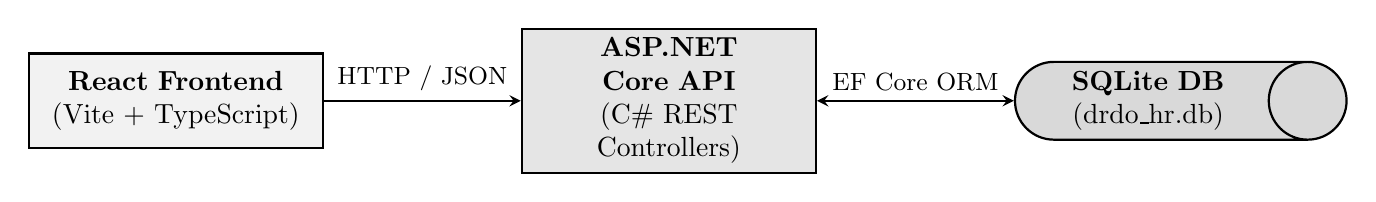
\begin{tikzpicture}[node distance=2cm, auto, >=stealth,
    block/.style={rectangle, draw=black, fill=gray!10, thick, text width=3.5cm, align=center, minimum height=1.2cm},
    cloud/.style={rectangle, draw=black, fill=gray!20, thick, text width=3.5cm, align=center, minimum height=1.2cm},
    db/.style={cylinder, draw=black, fill=gray!30, thick, text width=2.8cm, align=center, minimum height=1.5cm}]
    
    \node [block] (client) {\textbf{React Frontend}\\(Vite + TypeScript)};
    \node [cloud, right=2.5cm of client] (api) {\textbf{ASP.NET Core API}\\(C\# REST Controllers)};
    \node [db, right=2.5cm of api] (database) {\textbf{SQLite DB}\\(drdo\_hr.db)};
    
    \draw[->, thick] (client) -- node[above, font=\small] {HTTP / JSON} (api);
    \draw[<->, thick] (api) -- node[above, font=\small] {EF Core ORM} (database);
\end{tikzpicture}
\caption{Decoupled Client-Server System Architecture}
\end{figure}

\subsection{2.2 Database Data Models}

\begin{table}[htbp]
\centering
\caption{TIMP Database Schema Definitions}
\small
\renewcommand{\arraystretch}{1.5}
\begin{tabular}{|l|l|l|l|}
\hline
\textbf{Table Name} & \textbf{Field} & \textbf{Type} & \textbf{Description} \\ \hline
\multirow{4}{*}{\textbf{Users}} 
 & Id & int (PK) & Unique primary key identifier \\ \cline{2-4}
 & Email & string & Institutional email (@sspl.drdo.in) \\ \cline{2-4}
 & PasswordHash & string & BCrypt hashed password string \\ \cline{2-4}
 & Role & string & System access role (`admin`, `mentor`) \\ \hline
\multirow{5}{*}{\textbf{Interns}} 
 & Id & int (PK) & Candidate registration ID \\ \cline{2-4}
 & Name & string & Candidate full name \\ \cline{2-4}
 & Branch & string & Academic discipline \\ \cline{2-4}
 & Status & string & Candidate status (`New`, `Active`, etc.) \\ \cline{2-4}
 & MentorName & string & Assigned SSPL scientist mentor \\ \hline
\end{tabular}
\end{table}

% ==========================================
% PAGE 17-22: BACKEND API IMPLEMENTATION
% ==========================================
\newpage
\section{BACKEND REST API IMPLEMENTATION}

\subsection{3.1 Authentication Controller}
The `AuthController` manages candidate and administrative sign-in requests, authenticating users against BCrypt hashes and generating signed JWT tokens.

\begin{lstlisting}[language=csh, caption={C\# ASP.NET Core AuthController Implementation}]
[ApiController]
[Route("api/[controller]")]
public class AuthController : ControllerBase
{
    private readonly AppDbContext _context;
    private readonly IConfiguration _config;
    
    public AuthController(AppDbContext context, IConfiguration config)
    {
        _context = context;
        _config = config;
    }
    
    [HttpPost("login")]
    public IActionResult Login([FromBody] LoginRequest request)
    {
        if (string.IsNullOrWhiteSpace(request?.Email) || string.IsNullOrWhiteSpace(request?.Password))
            return BadRequest(new { message = "Email and password are required" });

        var inputEmail = request.Email.Trim().ToLowerInvariant();
        var trimmedPassword = request.Password.Trim();

        var user = _context.Users.AsEnumerable()
                    .FirstOrDefault(u => u.Email.Equals(inputEmail, StringComparison.OrdinalIgnoreCase));
        
        if (user == null)
            return Unauthorized(new { message = "Invalid email or password" });

        bool passwordValid = false;
        try {
            if (!string.IsNullOrEmpty(user.PasswordHash) && user.PasswordHash.StartsWith("$2"))
                passwordValid = BCrypt.Net.BCrypt.Verify(trimmedPassword, user.PasswordHash);
        } catch { }

        if (!passwordValid)
            passwordValid = (user.PasswordHash == trimmedPassword);

        if (!passwordValid)
            return Unauthorized(new { message = "Invalid email or password" });

        return GenerateJwtResponse(user);
    }
}
\end{lstlisting}

% ==========================================
% PAGE 23-29: FRONTEND UI & COMPONENTS
% ==========================================
\newpage
\section{FRONTEND UI \& COMPONENT IMPLEMENTATION}

\subsection{4.1 Axios API Client}
A centralized Axios client (`axiosInstance.ts`) handles API URL normalization, trailing slash sanitization, and automatic JWT Bearer token header injection.

\begin{lstlisting}[language=csh, caption={TypeScript Axios Client Implementation}]
import axios from 'axios';

let rawBaseURL = import.meta.env.VITE_API_URL || 'http://localhost:5000/api';
rawBaseURL = rawBaseURL.trim().replace(/\/+$/, '');
if (!rawBaseURL.endsWith('/api')) {
  rawBaseURL = `${rawBaseURL}/api`;
}

const api = axios.create({
  baseURL: rawBaseURL,
  headers: { 'Content-Type': 'application/json' }
});

api.interceptors.request.use((config) => {
  const token = localStorage.getItem('token');
  if (token) {
    config.headers.Authorization = `Bearer ${token}`;
  }
  return config;
});

export default api;
\end{lstlisting}

% ==========================================
% PAGE 30-34: DEPLOYMENT & CONCLUSION
% ==========================================
\newpage
\section{CLOUD DEPLOYMENT AND CONCLUSION}

\subsection{5.1 Docker Containerization Strategy}
The ASP.NET Core backend is containerized using a multi-stage Docker build pipeline based on official .NET 9.0 / .NET 8.0 LTS runtime images.

\begin{lstlisting}[language=docker, caption={Multi-Stage Backend Dockerfile}]
FROM mcr.microsoft.com/dotnet/sdk:9.0 AS build
WORKDIR /app

COPY *.csproj ./
RUN dotnet restore

COPY . ./
RUN dotnet publish -c Release -o out

FROM mcr.microsoft.com/dotnet/aspnet:9.0
WORKDIR /app
COPY --from=build /app/out .
RUN mkdir -p wwwroot/uploads

EXPOSE 10000
ENV ASPNETCORE_URLS=http://+:10000
ENTRYPOINT ["dotnet", "backend.dll"]
\end{lstlisting}

\subsection{5.2 Conclusion}
The **Trainee \& Internship Management Portal (TIMP)** project achieved all technical and functional milestones set by the HR and Systems Division at SSPL DRDO. The platform successfully automates paper-based intern tracking, provides real-time scientist allocation, enables visual attendance heatmap tracking, and facilitates print-ready DRDO certificate generation.

Future developments will focus on biometric smart-card integration and cloud PostgreSQL cluster migration.

\end{document}
